\documentclass[conference]{IEEEtran}
\usepackage{color}
\usepackage{tikz}
\usepackage{pstricks}

% Terri's simple FIXME macro
\newcommand{\FIXME}[1]{\textcolor{red}{FIXME: #1}}

% Tikz setup
\usetikzlibrary{arrows,decorations,decorations.text,decorations.pathreplacing,shapes}
\tikzstyle{box} = [rectangle, draw, text width=8em]
\tikzstyle{thread} = [rectangle, draw, minimum width=1em, minimum height=1em, fill=blue!40]
\tikzstyle{thread-cloud} = [cloud, draw, cloud puffs=10,cloud puff arc=120, aspect=2, inner ysep=1em, minimum width=16em, minimum height=12em]

\begin{document}
\title{Automated Proactive Software Hardening\\ through Fuzz Testing and Evolutionary Computation}

\author{}
%\author{\IEEEauthorblockN{Michael Shell}
%\IEEEauthorblockA{School of Electrical and\\Computer Engineering\\
%Georgia Institute of Technology\\
%Atlanta, Georgia 30332--0250\\
%Email: http://www.michaelshell.org/contact.html}
%\and
%\IEEEauthorblockN{Homer Simpson}
%\IEEEauthorblockA{Twentieth Century Fox\\
%Springfield, USA\\
%Email: homer@thesimpsons.com}
%\and
%\IEEEauthorblockN{James Kirk\\ and Montgomery Scott}
%\IEEEauthorblockA{Starfleet Academy\\
%San Francisco, California 96678-2391\\
%Telephone: (800) 555--1212\\
%Fax: (888) 555--1212}}

\maketitle

\begin{abstract}
Hardening software to make it more robust and able to withstand attacks can be
very challenging.  This paper explores a method for automated hardening by
combing an automated bug-finding technique with automated software
repair in a closed loop automated software hardening tool.  We
demonstrate the effectiveness of this approach through proactive
defeat of withheld real-world exploits.
\end{abstract}

\section{Introduction}
In their 2006 paper, Miller et al were disappointed to find that the robustness
of command line utilities on MacOS in 2006 than the Linux/GNU tools of 1995
\cite{Miller2006}.  While fuzz testing is a well-established technique for
testing software robustness, applying it to an existing project and then fixing
the bugs found as a result of this techinque takes time.  Unfortunately,
developers already can find more bugs than they realistically have time to fix
\cite{devshavetoomanybugs}.  \FIXME{blah blah about bugs, use citations from
previous genprog papers.}

However, it is now possible to use automated repair to fix bugs rather than
relying on human programmers.  This has proven to be very competitive, with one
study finding that bugs could be repaired for approximately \$8 per bug
\cite{manybugs}. \FIXME{some paragraph about genprog here, or maybe later?}

So we have an automated way to find bugs and an automated way to fix them: is it
possible to combine the two to proactively ``harden" software? 


\section{Technical Approach}

\begin{figure*}[htb]
  \centering
  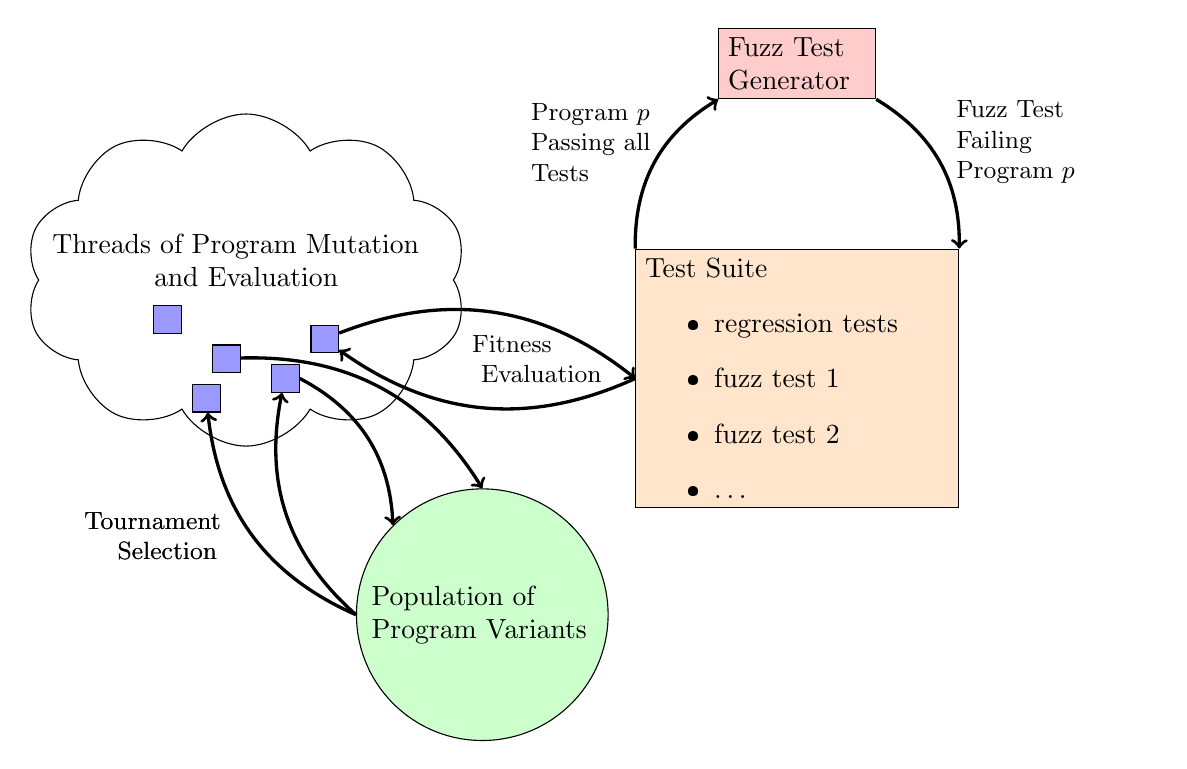
\begin{tikzpicture}[scale=0.5]
    \node [box, fill=red!20, text width=5em] (fuzz) at (6,2) {Fuzz Test\\Generator};
    \node [text width=14em] (genprog) at (-8,-3) {Threads of Program Mutation\\\centerline{and Evaluation}};
    \node [box, circle, fill=green!20] (pop) at (-2,-12) {Population of\\ Program Variants};
    \node [box, text width=11em, fill=orange!20] (test) at (6, -6)
    {Test Suite
      \begin{itemize}
      \item regression tests
      \item fuzz test 1
      \item fuzz test 2
      \item \ldots{}
      \end{itemize}};
    \node [thread-cloud] at (-8,-3.5) {};
    \node [thread] (t1) at (-9,-6.5) {};
    \node [thread] (t2) at (-7,-6) {};
    \node [thread] (t3) at (-6,-5) {};
    \node [thread] (t4) at (-10,-4.5) {};
    \node [thread] (t5) at (-8.5,-5.5) {};

    % population <-> threads
    \draw [->,very thick,bend left] (pop.west) to (t1);
    \draw [->,very thick,bend left] (pop.west) to (t2);
    \draw [->,very thick,bend left] (t5) to (pop.north);
    \draw [->,very thick,bend left] (t2.east) to (pop.north west);
    % threads <-> test
    \draw [->,very thick,bend left] (t3) to (test.west);
    \draw [->,very thick,bend left] (test.west) to (t3);
    % test <-> fuzz generator
    \draw [->,very thick,bend left] (test.north west) to (fuzz.south west);
    \draw [->,very thick,bend left] (fuzz.south east) to (test.north east);

    % arrow labels
    \node [text width=6em, font=\small] at (-10,-10) {Tournament\\\centerline{Selection}};
    \node [text width=6em, font=\small] at (-10,-10) {Tournament\\\centerline{Selection}};
    \node [text width=5em, font=\small] at (-0.5,-5.5) {Fitness\\\centerline{Evaluation}};
    \node [text width=5em, font=\small] at (1,0) {Program $p$ Passing all Tests};
    \node [text width=7em, font=\small] at (12.5,0) {Fuzz Test\\Failing\\Program $p$};
  \end{tikzpicture}
  
  \caption{Overview of Fuzz Hardening framework}
  \label{fig:overview}
\end{figure*}

\subsection{Fuzz Testing}

Fuzz testing is a software testing technique used to find bugs due to unexpected
input.  Fuzz testers range from the original work using purely random characters
\cite{Miller1990,Miller1995} to input that is very specifically tweaked from a
template or grammar \cite{modern,fuzz,papers}, or even randomized input that
includes mouse or window events \cite{Miller2006}.

For our experiments, we started with the most basic fuzz tester,
as provided by Miller as fuzz-2001 \cite{Millerfuzzwebsite}, which generates
different lengths of files filled with randomized characters.  These early
experiments explored whether even a fairly modest fuzzer could be used to
produce useful software hardening, and this is the most basic fuzz tester
available.

Later experiments used a more advanced block-based network fuzzer called SPIKE
\cite{SPIKE}.  Rather than generating purely randomized data, SPIKE uses a block
structure that can be used to give it a notion of syntax for communicating.
The fuzzer modifies variable areas of the protocol while leaving the essential
command structure intact.  In addition, the parts that are fuzzed use not only
random data, but also some heuristically chosen strings that often cause
problems in software. 

\FIXME{More about possible fuzz testers for future work, incl. Flayer}


\subsection{Automated Software Repair}

For the automated software repair part of the system, we have used a lisp
implementation of Genprog \cite{genprogpapers}.   This particular version of
genprog was easier to script for repeated repairs.  \FIXME{more here}

\subsection{Automated hardening procedure}

\begin{figure}[htb]
  \caption{Automated Hardening Procedure}
  \label{fig:flowchart}
  \centering
    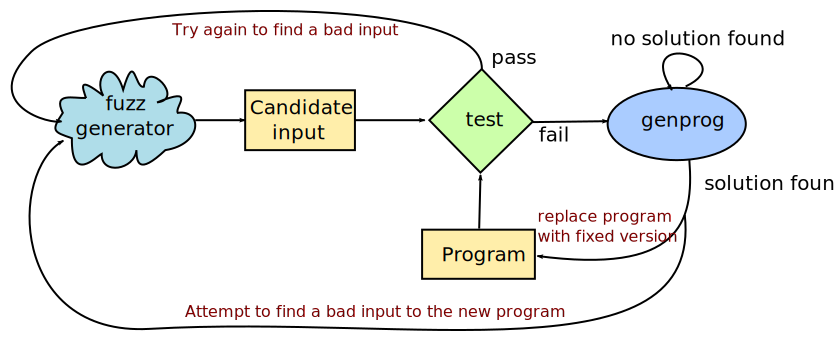
\includegraphics[width=0.5\textwidth]{automated-hardening-simple.eps}
%\input{automated-hardening-simple.tex}
\end{figure}


Figure~\ref{fig:flowchart} shows the procedure used for automated hardening.  We
start with the fuzz generator, which is used to produce a candidate input.
This candidate output is then run as input to the program which we are
attempting to harden.  If the program passes on that input, we go back to the
fuzz generator and continue to generate candidates until we get one that fails.
In this case, a failing candidate input is one that causes the program to hang
or crash.  Once a failing candidate input is found, genprog is engaged to find a
new version of the program that does not fail on the candidate input.  Genprog
is run until it finds a solution, at which point that solution replaces the
program being hardened and we create a new test case using the previously
failing input.  We can then return to the beginning of the process and start
finding a new candidate input.

There are a couple of places which require timeouts: 

\begin{enumerate}
\item At the candidate input
generation phase, we need to set a limit on the amount of time spent trying to
find a new failing input.  If no failing inputs are found within that time,
terminate the run on the assumption that the program has been sufficiently
hardened against the fuzz tester.

\item At the genprog phase, it is possible that genprog will be unable to find
a repair for this failure.  Again, a timeout can be set so that genprog will be
terminated.  This could be after a given amount of time, generations of the
program population, or number of random seeds used to initiatlize genprog.  At
this point, that candidate input could be given to a human programmer to
analyse, while the system returns to finding new candidate inputs that may be
more repairable.
\end{enumerate}

Our choice of what it means to ``fail" a test is fairly simplistic: we assume a
failure means a crash or hang of the program.  This is appropriate for some
types of program, such as server software where a crash or hang would cause the
server to become unresponsive to other requests.   For other types of programs
other failure criteria might be necessary. 

Note also that it is very hard to determine an optimal solution from a failing
fuzzed input.  The ASH system attempts to produce a new program that does not
crash, but it might be more appropriate for the system to generate an
appropriate error message, log the attempt to input malformed data, or other
action.  If this action can be predicted in advance, such as a standard error
message that needs to be returned, it is possible to add this desired action
into the test cases generated by ASH and sent to genprog so it will generate a
program behaves as desired.   Unfortunately, this may not generate very
informative messages and behaviours, but it could be "good enough" until a human
programmer can create a more informed test case or patch to the program.



\section{Conclusion}
We have produced a system that combines the bug-finding utility of a fuzz tester
with the patch-finding ability of automated repair system genprog.


\section{Availability}
\FIXME{Is Eric's code released?  We should release our linking scripts and
SPIKE scripts in some useful way.}

\section*{Acknowledgment}

The authors would like to thank...
- DARPA

\bibliographystyle{IEEEtran}
\bibliography{pst2013.bib}

\end{document}
